%!TEX TS-program = xelatex
\documentclass[]{friggeri-cv}
\usepackage{afterpage}
\usepackage{pifont}
\usepackage{hyperref}
\usepackage{color}
\usepackage{eurosym}
\usepackage{xcolor}
\usepackage{array}
\hypersetup{
    pdftitle={},
    pdfauthor={},
    pdfsubject={},
    pdfkeywords={},
    colorlinks=false,       % no lik border color
   allbordercolors=white    % white border color for all
}
%\addbibresource{bibliography.bib}
\RequirePackage{xcolor}
\definecolor{pblue}{HTML}{0395DE}

\begin{document}
\header{\hspace{1.2cm}George}{Evangelopoulos}
        {Computer Engineer}
      
% Fake text to add separator      
\fcolorbox{white}{gray}{\parbox{\dimexpr\textwidth-2\fboxsep-2\fboxrule}{%
.....
}}

% In the aside, each new line forces a line break
\begin{aside}
  \section{Address\\}
    Dardanelion 3, 55131\\
    Thessaloniki, Greece\\
 
  \section{Tel \& Skype\\}
    +30 697 897 9684\\
    evangelopoulos.george\\
    
  \section{Mail, Web \& Git}
    \href{mailto:evangelopoulos.george@gmail.com}{\textbf{evangelopoulos.george@}\\gmail.com}\\
    \href{https://www.linkedin.com/in/gevangelopoulos}{\raisebox{-0.2\height}{
\includegraphics[scale=0.05]{img/Linkedin}}/gevangelopoulos}\\
    \href{https://github.com/gevangelopoulos}{\raisebox{-0.2\height}{
\includegraphics[scale=0.06]{img/Github}}/gevangelopoulos}\\
   
  \section{Programming\\}
%    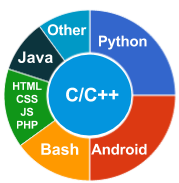
\includegraphics[scale=0.62]{img/programming.png}
    \vspace{0.3cm}
        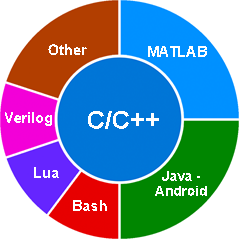
\includegraphics[scale=0.95]{img/cv_languages.pdf}\\
        
  \section{OS Preference\\}
    \textbf{GNU/Linux}\raisebox{-0.2\height}{
\includegraphics[scale=0.40]{img/5stars.png}}\\
    \textbf{Bare Metal}\raisebox{-0.2\height}{
\includegraphics[scale=0.40]{img/4stars.png}}\\
    \textbf{Unix-like}\raisebox{-0.2\height}{
\includegraphics[scale=0.40]{img/3stars.png}}\\
    \textbf{Windows}\raisebox{-0.2\height}{
\includegraphics[scale=0.40]{img/2stars.png}}\\
    
      \section{Tools\\}
    \vspace{0.2cm}
    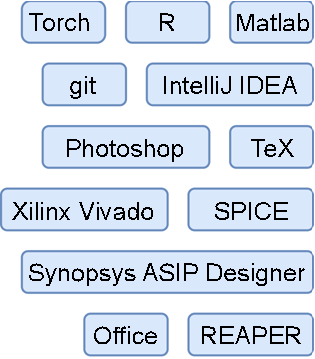
\includegraphics[scale=0.6]{img/cv_skills.pdf}
   
  \section{Most Proud Of\\}
  Top 5\% of my class \color{pblue}{\ding{51}}\\ 
  Organized a 1500+ \\participant conference \ding{51}\\
  Raised over \EUR10k \\for student NGOs \ding{51}\\
  Served in the Military \ding{51}\\
  
    \section{Languages\\}
  \renewcommand*{\arraystretch}{0.1}
  \begin{tabular}{c@{\hskip 0.1cm}c@{\hskip 0.1cm}c@{\hskip 0.1cm}c}
  	
\includegraphics[scale=0.3]{img/Greece.png} & 
\includegraphics[scale=0.3]{img/United-Kingdom.png}& 
\includegraphics[scale=0.3]{img/France.png} & 
\includegraphics[scale=0.3]{img/Germany.png}\\ 
  	\textbf{\color{pblue}{N}}&\textbf{\color{pblue}{C2}}&\textbf{B2}&\textbf{B1}  
  \end{tabular} 
   


\end{aside}

\section{Education}
\begin{entrylist}
	\entry
	{2010 - 2016}
	{M. Eng. in Electrical \& Computer Engineering}
	{\\Aristotle University of Thessaloniki, Greece}
	{\emph{GPA: 8.51/10 "Excellent", top 5\% of 243}\\
		Specialization Electronics and Computer Engineering\\
		Main subjects: Microelectronics, Microprocessors, Control Theory, Operating Systems, Software Engineering, Networks \& Databases
		}
%	\entry
%	{2005 - 2009}
%	{Bachelor's Degree in Computer Engineering}
%	{Università di Pisa, Italy}
%	{Main subjects: Matematics and Physics, Programming, Operational Research, Telecommunication Systems, Digital and Analogical Electronics.\\
%		\emph{Title of the Thesis: "Development, Management and Migrations of web contents and applications".}\\
%		\emph{Thesis activity carried out during an internship period at Atitlan Engineering SRL.}\\}
%	\entry
%	{2000 - 2005}
%	{Scientific Disploma.}
%	{Liceo Scientifico, Matera, Italy}
%	{Scientific Secondary School.\\
%		Main subjects: Matematics, Physics, Computer Science.}
\end{entrylist}

\vspace{-\parsep}
\section{Research}
\vspace{-\parsep}
\begin{entrylist}
	\entry
	{02/16 - 06/16}
	{Master Thesis}
	{KU Leuven, Belgium}
	{Efficient Hardware Mapping of LSTM Neural Networks for Automatic Speech Recognition\vspace{0.5\baselineskip}
	\begin{itemize}
		\item Developed, trained and tested an LSTM architecture in Torch 7
		\item Optimized for hardware by modeling fixed-precision arithmetic, network connection pruning and coarse activation functions in MATLAB 
		\item Modified an ASIP architecture for LSTMs in Synopsis ASIP Designer, achieving energy savings up to 80\%
\end{itemize}
\emph{Supervisors: Prof. dr. ir. Marian Verhelst, Ir. Bert Moons}}

\entry
{09/15 - 01/16}
{Graduate Student Researcher}
{York University, Canada}
{Development of a Signal Detector for Nanopore-based DNA Sequencing\vspace{0.5\baselineskip}
	\begin{itemize}
		\item Developed event-detection algorithms in C for automated DNA sequencing from data gathered from an Oxford-Nanopore MinION sensor
		\item Implemented, tested and deployed on an ARM-FPGA architecture (Xilinx ZYNQ) using Verilog and High Level Synthesis
		\item Demonstrated realtime behavior and large energy savings
\end{itemize}
\emph{Supervisor: Prof. Sebastian Magierowski}}
\end{entrylist}

\vspace{-\parsep}
\section{Experience}
\vspace{-\parsep}
\begin{entrylist}
    \entry
    {07/16 - 11/16}
    {Software Developer}
    {UnifyID, San Francisco, CA, USA}
    {Designed and developed the company's Android application by implementing its REST API, Amazon AWS connectivity, crypto and user interface.}
    \entry
    {08/14 - 08/15}
    {Web Developer}
    {DatAnalysis, Thessaloniki, Greece}
    {Designed, developed and managed a website of a construction company on Drupal 7 and an e-commerce website on Magento 1.9.}
    \entry
    {07/14 - 12/14}
    {Electrical Engineering Internship}
    {SELI - AEGEK CJV, Thessaloniki, Greece}
    {Configured and maintained PLC-based machinery, medium/low voltage transmission lines, transformers and circuitry used in the construction of Thessaloniki's metro.}
\end{entrylist}
\vspace{-\parsep}
\section{Volunteer Experience}
\vspace{-\parsep}
\begin{entrylist}
	\entry
	{05/13 - 04/14}
	{Project Coordinator}
	{ECE Student Conference 7, Thessaloniki, Greece}
	{Led a group of 20 to organize the 7th panhellenic conference for ECE students, with 50+ presentations and 1500+ participants.}
  \entry
    {10/12 - 10/14}
    {Vice-President of Fundraising}
    {Local BEST Group, Thessaloniki, Greece}
    {Led and motivated a group of 40, managing and coordinating the organization of various international events, seminars and competitions for engineering students. }
\end{entrylist}
%\section{Certifications}
%\begin{entrylist}
%  \entry
%    {02/2013}
%    {Intro to Computer Science}
%    {Udacity. E-learning}
%    {\emph{Building a Python Search Engine}}
%\end{entrylist}

%\newpage
%
%\begin{aside}
%~
%~
%~
%  \section{Places Lived}
%    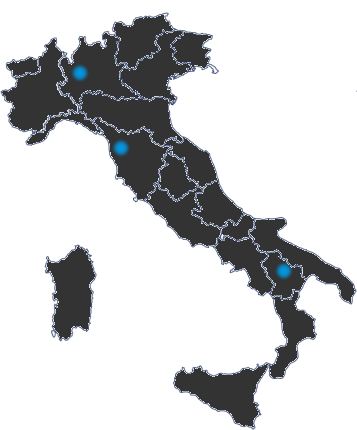
\includegraphics[scale=0.25]{img/italia.png}
%    ~
%  \section{Languages}
%    \textbf{Italian}
\includegraphics[scale=0.40]{img/5stars.png}
%    \textbf{English}
\includegraphics[scale=0.40]{img/4stars.png}
%\end{aside}

%\section{Publications}
%C. Benedetto, E. Mingozzi, C. Vallati\\
%\textbf{A Handoff Algorithm based on Link Quality Prediction for Mass Transit Wireless Mesh Networks}\\
%\emph{Proceedings of the 18th IEEE Symposium on Computers and Communications (ISCC 2013), Split, Croatia, July 7-10, 2013}
%\\
%\section{Other Info}
%For the Italian job market:\\
%\emph{Si autorizza il trattamento delle informazioni contenute nel curriculum in conformità alle disposizioni previste dal d.lgs. 196/2003. Si dichiara altresì di essere consapevole che, in caso di dichiarazioni non veritiere, si è passibili di sanzioni penali ai sensi del DPR 445/00 oltre alla revoca dei benefici eventualmente percepiti.}
%\\
%\begin{flushleft}
%\emph{January 14th, 2014}
%\end{flushleft}
%\begin{flushright}
%\emph{Carmine Benedetto}
%\end{flushright}

%%% This piece of code has been commented by Karol Kozioł due to biblatex errors. 
% 
%\printbibsection{article}{article in peer-reviewed journal}
%\begin{refsection}
%  \nocite{*}
%  \printbibliography[sorting=chronological, type=inproceedings, title={international peer-reviewed conferences/proceedings}, notkeyword={france}, heading=subbibliography]
%\end{refsection}
%\begin{refsection}
%  \nocite{*}
%  \printbibliography[sorting=chronological, type=inproceedings, title={local peer-reviewed conferences/proceedings}, keyword={france}, heading=subbibliography]
%\end{refsection}
%\printbibsection{misc}{other publications}
%\printbibsection{report}{research reports}
\end{document}
